\subsection{Spin und Pauli-Prinzip}
\label{subsec:spin_und_pauli_prinzip}

Neben Masse\index{Masse}, elektrischer Ladung\index{Ladung!elektrische} und
Wellencharakter\index{Wellencharakter!des Elektrons} besitzt das Elektron
\index{Elektron} eine weitere grundlegende Eigenschaft: den Spin\index{Spin}.
Der Spin ist eine rein quantenmechanische Eigenschaft. Er darf nicht einfach
als klassische Drehung des Elektrons um seine eigene Achse verstanden werden.

Anschaulich erinnert der Begriff zwar an eine Eigenrotation. Dieses Bild ist
aber nur begrenzt brauchbar. Das Elektron ist nach heutigem Verständnis kein
kleines Kügelchen mit einer ausgedehnten Oberfläche, die sich mechanisch drehen
würde. Der Spin gehört vielmehr direkt zum quantenmechanischen Zustand
\index{Zustand!quantenmechanischer} des Elektrons.

Für das Elektron beträgt die Spinquantenzahl\index{Spinquantenzahl}

\begin{equation}
	s = \frac{1}{2}
	\label{eq:spin_elektron}
\end{equation}

Misst man die Projektion des Spins auf eine gewählte Raumrichtung, so sind für
das Elektron nur zwei Werte möglich:

\begin{equation}
	m_s = +\frac{1}{2}
	\qquad \text{oder} \qquad
	m_s = -\frac{1}{2}
	\label{eq:spinprojektion_elektron}
\end{equation}

Diese beiden Möglichkeiten werden häufig vereinfacht als Spin nach oben und
Spin nach unten bezeichnet. Gemeint ist dabei nicht eine klassische Richtung
einer rotierenden Kugel, sondern ein möglicher Messwert der
Spinprojektion\index{Spinprojektion}.

\begin{PhysicsBox}[Spin des Elektrons]
	\label{box:spin_elektron}
	Der Spin ist eine intrinsische quantenmechanische Eigenschaft des Elektrons.
	Für das Elektron gilt \(s = 1/2\). Bei einer Messung der Spinprojektion sind
	nur zwei Werte möglich: \(m_s = +1/2\) und \(m_s = -1/2\).
\end{PhysicsBox}
\FloatBarrier

\begin{figure}[H]
	\centering
	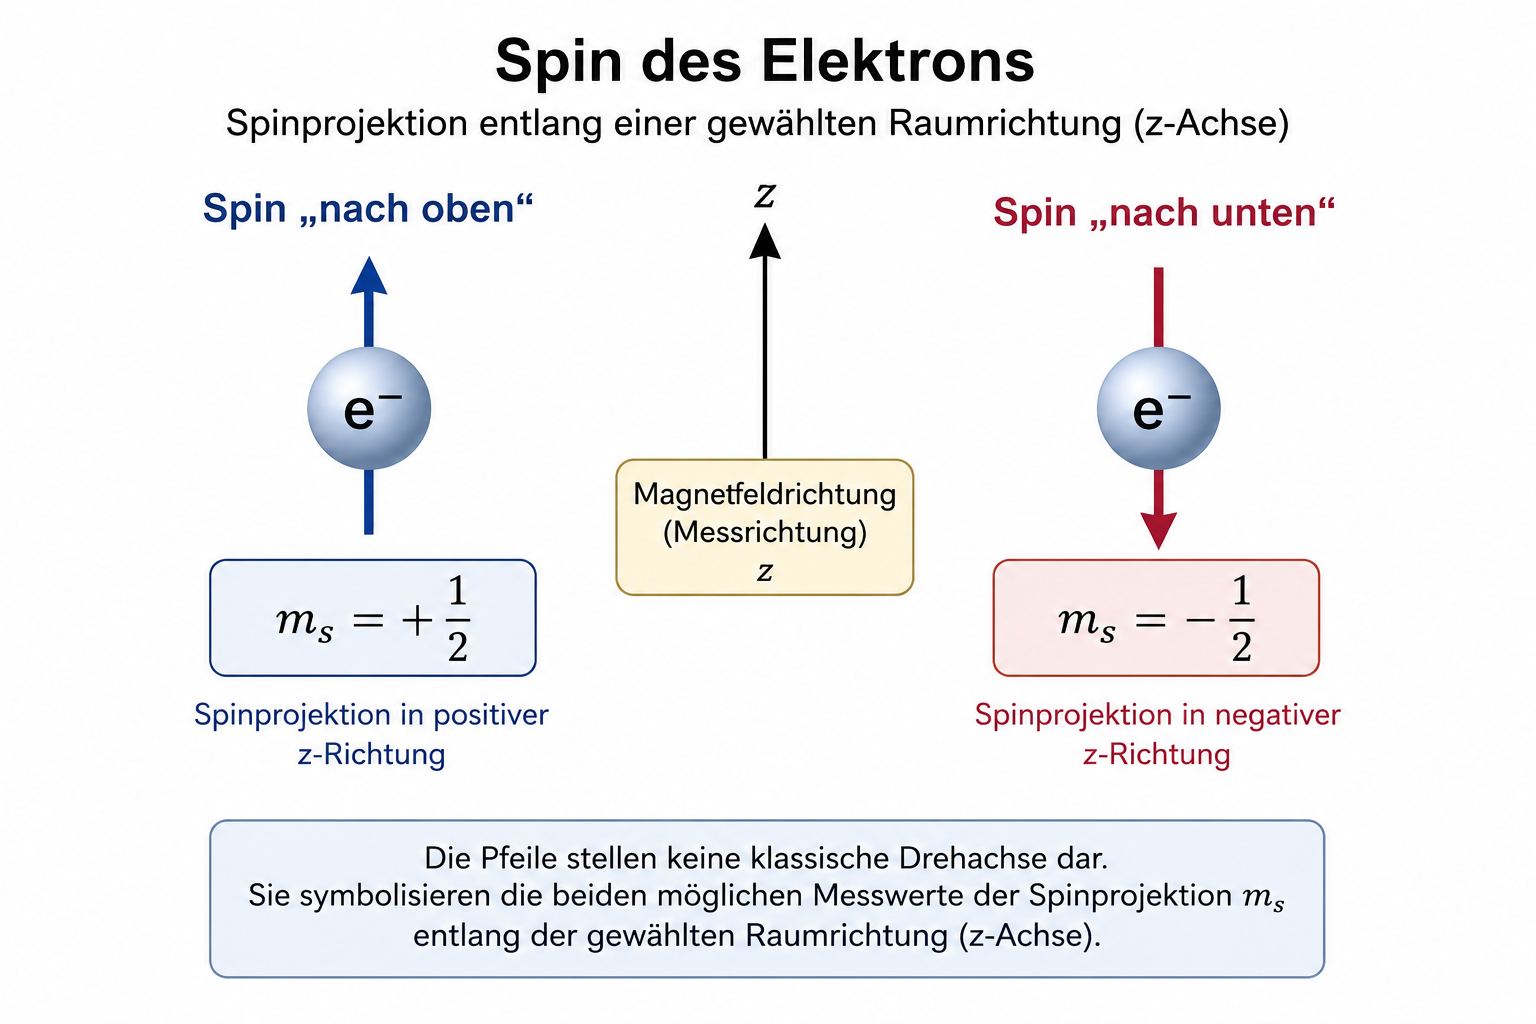
\includegraphics[width=0.75\textwidth]{bilder/spin}
	\caption{Schematische Darstellung der beiden möglichen Spinprojektionen des
		Elektrons. Die Pfeile stehen nicht für eine klassische Drehbewegung, sondern
		für die möglichen Messwerte \(m_s = +1/2\) und \(m_s = -1/2\) entlang einer
		gewählten Raumrichtung.}
	\label{fig:spin_elektron}
\end{figure}




Der Spin hat wichtige physikalische Folgen.

Der Spin hat wichtige physikalische Folgen. Da das Elektron elektrisch geladen
ist, ist mit seinem Spin auch ein magnetisches Moment
\index{magnetisches Moment} verbunden. Dadurch verhält sich das Elektron in
magnetischen Feldern\index{magnetisches Feld} so, als besäße es einen kleinen
magnetischen Charakter. Dies spielt unter anderem bei der Struktur von Atomen,
bei magnetischen Eigenschaften von Stoffen und in der modernen Messtechnik eine
wichtige Rolle.

Besonders entscheidend wird der Spin im Zusammenhang mit dem
Pauli-Prinzip\index{Pauli-Prinzip}. Wolfgang Pauli\index{Pauli, Wolfgang}
formulierte 1925 ein Ausschließungsprinzip für Elektronen in Atomen. Er kam
nicht durch ein anschauliches mechanisches Modell darauf, sondern durch die
Analyse atomarer Spektren\index{Atomspektrum} und der Ordnung des
Periodensystems\index{Periodensystem}.

Die damals bekannten Quantenzahlen reichten nicht aus, um die beobachteten
Regelmäßigkeiten vollständig zu erklären. Pauli erkannte, dass Elektronen in
einem Atom nicht beliebig denselben Zustand besetzen können. Jeder vollständig
beschriebene Elektronenzustand darf in einem Atom nur einmal vorkommen. Erst
später wurde klar, dass die zusätzliche Zweideutigkeit der Elektronenzustände
mit dem Spin des Elektrons zusammenhängt.

Das Pauli-Prinzip besagt:

\begin{equation}
	\begin{aligned}
		&\text{Keine zwei Elektronen eines Atoms dürfen in allen} \\
		&\quad \text{Quantenzahlen übereinstimmen.}
	\end{aligned}
	\label{eq:pauli_prinzip_text}
\end{equation}

Ein Elektron in einem Atom wird durch mehrere Quantenzahlen\index{Quantenzahl}
beschrieben. Dazu gehören die Hauptquantenzahl \(n\)\index{Hauptquantenzahl},
die Nebenquantenzahl \(l\)\index{Nebenquantenzahl}, die magnetische Quantenzahl
\(m_l\)\index{magnetische Quantenzahl} und die Spinquantenzahl \(m_s\)
\index{Spinquantenzahl}.

Ein Zustand eines Elektrons kann daher durch folgendes Schema beschrieben
werden:

\begin{equation}
	(n,\, l,\, m_l,\, m_s)
	\label{eq:quantenzahlen_elektron_zustand}
\end{equation}

Das Pauli-Prinzip fordert also, dass zwei Elektronen in einem Atom nicht
dieselbe Kombination dieser vier Quantenzahlen besitzen dürfen. Das bedeutet:
Zwei Elektronen dürfen nicht im vollständig gleichen quantenmechanischen
Zustand sein.

Anschaulich wird dies am einfachsten an einem einzelnen Orbital. Ein Orbital
\index{Orbital} ist durch die drei Quantenzahlen \(n\), \(l\) und \(m_l\)
festgelegt. Diese drei Quantenzahlen beschreiben die Schale, die Form und die
räumliche Orientierung des Orbitals. Für den Spin bleibt dann noch die vierte
Quantenzahl \(m_s\).

Betrachten wir als Beispiel das \(1s\)-Orbital\index{1s-Orbital}. Es wird durch
die Quantenzahlen

\begin{equation}
	n = 1, \qquad l = 0, \qquad m_l = 0
	\label{eq:quantenzahlen_1s_orbital}
\end{equation}

beschrieben. Für ein Elektron in diesem Orbital sind nun nur zwei verschiedene
Spinwerte möglich:

\begin{equation}
	m_s = +\frac{1}{2}
	\qquad \text{oder} \qquad
	m_s = -\frac{1}{2}
	\label{eq:spinwerte_1s_orbital}
\end{equation}

Damit können im \(1s\)-Orbital höchstens zwei Elektronen sitzen. Ihre
Quantenzahlen lauten dann:

\begin{equation}
	\left(1,\,0,\,0,\,+\frac{1}{2}\right)
	\qquad \text{und} \qquad
	\left(1,\,0,\,0,\,-\frac{1}{2}\right)
	\label{eq:zwei_elektronen_1s}
\end{equation}

Ein drittes Elektron könnte in diesem Orbital keinen neuen Spinwert mehr
annehmen. Es müsste daher dieselbe Kombination aller vier Quantenzahlen besitzen
wie eines der beiden bereits vorhandenen Elektronen. Genau das verbietet das
Pauli-Prinzip.

\begin{PhysicsBox}[Folge des Pauli-Prinzips]
	\label{box:pauli_prinzip_orbital}
	Ein Orbital kann maximal zwei Elektronen aufnehmen. Diese beiden Elektronen
	besitzen dieselben räumlichen Quantenzahlen \(n\), \(l\) und \(m_l\), müssen
	sich aber in ihrer Spinquantenzahl \(m_s\) unterscheiden.
\end{PhysicsBox}

Damit wird verständlich, warum die Elektronenhülle\index{Elektronenhülle} eines
Atoms eine geordnete Struktur besitzt. Die Elektronen können nicht alle
denselben Zustand einnehmen. Sie müssen sich auf verschiedene
quantenmechanische Zustände verteilen. Aus dieser Verteilung entstehen Schalen
\index{Schale!Atom}, Unterschalen\index{Unterschale} und die typische Ordnung
des Periodensystems.

Das Pauli-Prinzip ist deshalb eine der Grundlagen für den Aufbau der Materie
\index{Materie}. Ohne dieses Prinzip würden Elektronen in Atomen nicht die
beobachtete Schalenstruktur bilden. Die chemischen Eigenschaften der Elemente
\index{chemisches Element}, die Stabilität der Materie und viele Eigenschaften
von Festkörpern\index{Festkörper} hängen direkt mit diesem Prinzip zusammen.

Spin und Pauli-Prinzip verbinden damit die Quantenmechanik des einzelnen
Elektrons mit der Struktur ganzer Atome. Sie erklären, warum Elektronen nicht
beliebig Zustände besetzen können und warum aus wenigen quantenmechanischen
Regeln die Ordnung der Atomhülle entsteht.